\documentclass[11pt,a4paper]{article}
\usepackage{tikz}
\usetikzlibrary{arrows.meta,positioning}
\usepackage{tabularx}
\usepackage{amsmath,amssymb,amsthm}
\usepackage{geometry}
\geometry{margin=1in}
\usepackage{hyperref}
\usepackage{graphicx}
\usepackage{setspace}
\onehalfspacing

\title{\textbf{Paper D-02: Pandemic Dynamics:\\ A Constraint-Driven Flux Dynamics (CDFD) Perspective}}
\author{Steve Bico Mujjabi, MD\\
\small Independent Researcher\\
\small Founder, Vura Labs\\
\small Kampala, Uganda\\
\small ORCID: 0009-0001-0556-5516}
\date{August 2026}

\begin{document}
\maketitle

% BEGIN SHARED-METHODS POINTER
\noindent\textit{Shared Part IV notation and evidence boundaries are defined in \path{PART_IV_METHODS_AND_CLAIM_BOUNDARY.md}. This paper states only its local observables, comparison, and failure conditions.}
% END SHARED-METHODS POINTER


\begin{abstract}
This paper develops a falsifiable CDFD/AFL model of Pandemic Dynamics. It maps infection, contact, mobility, and pathogen replication to driving flux $\Phi$, susceptibility, immunity, behavior, healthcare, and surveillance capacity to active constraint $C$, vaccination, behavior change, treatment, tracing, and system expansion to responsiveness $S$, and immune history, trust, prior waves, infrastructure, and policy legacy to structural memory $M_s$. The target outcome is incidence, severity, burden, spread, and recovery, tested against epidemiology, mobility, genomics, serology, healthcare load, and intervention records. The paper treats universality as a shared model architecture rather than an assertion that unlike systems have the same material mechanism. It states the negative result that would make the mapping unnecessary and places the domain claim inside the cumulative CDFD programme and its reproducible runtime boundary.
\end{abstract}

\section{Introduction}

A pandemic is an informational virus spreading across a biological network. The pathogen attempts to maximize its throughput (transmission) by utilizing the host population's inherent social and economic connectivity. When the pathogen poses a mortal threat, the society behaves exactly like a single immune system: it deploys systemic constraints to block the flow.

CDFD models the society and the pathogen as a coupled fluid-mechanical system. The effectiveness of the public health response depends entirely on the topological elasticity of the population.

\section{The Epidemiological Adaptive Surface}
We govern the pandemic response using the Adaptive Operating Ratio:
\begin{equation}
    \Psi_s = \left( \frac{\Phi}{C} \right) \cdot S \cdot M_s
\end{equation}

For a society under viral threat:
\begin{itemize}
    \item \textbf{Flux ($\Phi$)}: The viral transmission rate (closely related to $R_0$) and the raw volume of human-to-human contact.
    \item \textbf{Constraint ($C$)}: Quarantines, mask mandates, border closures, and eventually, vaccination walls. These are artificial barriers erected to drive $\Phi$ to zero.
    \item \textbf{Responsiveness ($S$)}: The healthcare system capacity. The number of ICU beds, ventilators, and medical personnel able to absorb and process the severe cases generated by the flux.
    \item \textbf{Memory ($M_s$)}: Societal fatigue and institutional adherence. High memory implies strict, unwavering adherence to the constraint mandates. As memory degrades over time (lockdown fatigue), the constraints effectively weaken.
\end{itemize}

\subsection{Lockdown Fatigue and Pandemic Waves}
At the onset of a deadly pandemic, the pathogen flux $\Phi$ is extremely high. The society's responsiveness $S$ (hospitals) begins to saturate. To prevent the system from entering a catastrophic over-flux state ($\Psi_s \gg 1$), the government mandates a lockdown, instantly driving the constraint $C$ to an extreme high. The effective flux $\Phi$ drops, and the system stabilizes.

However, strict lockdowns are fundamentally unnatural to a highly connected socioeconomic surface. Maintaining high $C$ causes economic necrosis (as described in the Socioeconomic CDFD papers). Over months, societal memory $M_s$ degrades. The populace ceases to adhere strictly to the mandates. The effective constraint $C$ drops, and because the pathogen is still present, the flux $\Phi$ surges again. This triggers the classic "Second Wave" of the pandemic.



\section{Measurement Layer}

% BEGIN PART IV MAJOR CROSS-DOMAIN UPGRADE
\section{Cross-Domain Model Upgrade: Mechanism, Scale, and Tests}

\subsection{Observable Translation}

The paper-specific translation begins with an observable chain rather than a
verbal analogy. For Pandemic Dynamics, the proposed drive is infection, contact, mobility, and pathogen replication.
The active limitation is susceptibility, immunity, behavior, healthcare, and surveillance capacity. Responsiveness is carried by
vaccination, behavior change, treatment, tracing, and system expansion, while retained state is represented by
immune history, trust, prior waves, infrastructure, and policy legacy. The outcome to explain is incidence, severity, burden, spread, and recovery.

\begin{table}[htbp]
\centering
\small
\caption{Operational CDFD/AFL map for Paper D-02.}
\begin{tabularx}{\textwidth}{|l|X|X|}
\hline
\textbf{Term} & \textbf{Paper-specific observable meaning} & \textbf{Measurement question} \\
\hline
$\Phi$ & infection, contact, mobility, and pathogen replication & What rate, load, gradient, or demand enters the focal system? \\
\hline
$C$ & susceptibility, immunity, behavior, healthcare, and surveillance capacity & Which measured bottleneck limits transfer, function, or recovery? \\
\hline
$S$ & vaccination, behavior change, treatment, tracing, and system expansion & Which process changes effective capacity or reroutes the load? \\
\hline
$M_s$ & immune history, trust, prior waves, infrastructure, and policy legacy & Which retained state makes equal present loads produce different futures? \\
\hline
$Y$ & incidence, severity, burden, spread, and recovery & Which outcome is predicted out of sample, with uncertainty? \\
\hline
\end{tabularx}
\end{table}

\begin{figure}[htbp]
\centering
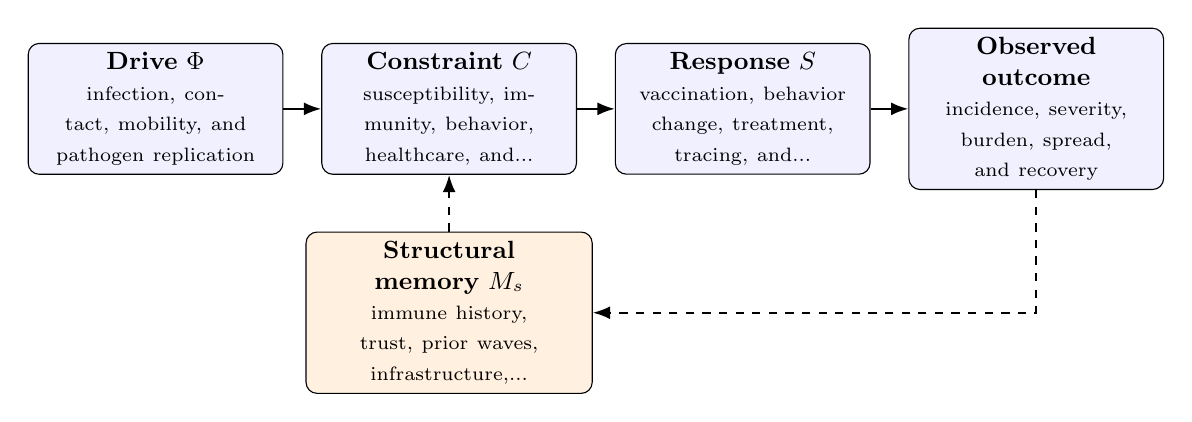
\begin{tikzpicture}[
    node distance=0.48cm,
    every node/.style={font=\small},
    box/.style={draw, rounded corners, align=center, minimum height=1.45cm, text width=3.0cm, fill=blue!6},
    memory/.style={draw, rounded corners, align=center, minimum height=1.25cm, text width=3.4cm, fill=orange!12},
    flow/.style={-{Latex[length=2.2mm]}, thick},
    feedback/.style={-{Latex[length=2.2mm]}, thick, dashed}
]
\node[box] (drive) {\textbf{Drive $\Phi$}\\\scriptsize infection, contact, mobility, and pathogen replication};
\node[box, right=of drive] (constraint) {\textbf{Constraint $C$}\\\scriptsize susceptibility, immunity, behavior, healthcare, and...};
\node[box, right=of constraint] (response) {\textbf{Response $S$}\\\scriptsize vaccination, behavior change, treatment, tracing, and...};
\node[box, right=of response] (outcome) {\textbf{Observed outcome}\\\scriptsize incidence, severity, burden, spread, and recovery};
\node[memory, below=0.72cm of constraint] (memory) {\textbf{Structural memory $M_s$}\\\scriptsize immune history, trust, prior waves, infrastructure,...};
\draw[flow] (drive) -- (constraint);
\draw[flow] (constraint) -- (response);
\draw[flow] (response) -- (outcome);
\draw[feedback] (outcome.south) |- (memory.east);
\draw[feedback] (memory.north) -- (constraint.south);
\end{tikzpicture}
\caption{Paper D-02 observable CDFD/AFL architecture for Pandemic Dynamics. Solid arrows give the proposed forward chain; dashed arrows make history-dependent feedback explicit.}
\label{fig:d02-architecture}
\end{figure}

\subsection{Paper-Specific Causal Hypothesis}

For this paper, the hypothesized causal sequence is specific. A change in
infection, contact, mobility, and pathogen replication arrives faster than vaccination, behavior change, treatment, tracing, and system expansion can compensate.
This raises or redistributes susceptibility, immunity, behavior, healthcare, and surveillance capacity. If the load persists,
the retained state encoded by immune history, trust, prior waves, infrastructure, and policy legacy changes the next response, so a later event of equal
magnitude can produce a different trajectory in incidence, severity, burden, spread, and recovery. The
scientific task is to estimate that sequence against the best ordinary model of
the domain, not merely to redescribe the outcome after it occurs.

\subsection{Cross-Scale Translation Without Mechanistic Erasure}

For the domain applications family, the cross-domain translation is a disciplined test across systems with very different material mechanisms. A valid mapping preserves the baseline science of the domain, declares the scale of every variable, and earns its place through a discriminating prediction rather than resemblance alone. \cite{Holling1973,Turing1952,Shannon1948,BakTangWiesenfeld1987}
The required scale declaration for this paper is hours to decades; hosts to global transmission networks. At short
scales, the key question is whether the incoming drive is transmitted,
buffered, or diverted. At intermediate scales, response changes effective
capacity and network exposure. At long scales, retained structure can alter the
state space itself. A result is genuinely cross-scale only when the aggregation
rule is stated and the same conclusion is not an artifact of averaging.

\subsection{Evidence Ladder and Discriminating Tests}

\begin{table}[htbp]
\centering
\small
\caption{Evidence ladder for Paper D-02. Each rung can fail independently.}
\begin{tabularx}{\textwidth}{|p{0.17\textwidth}|X|X|}
\hline
\textbf{Test} & \textbf{Design} & \textbf{Discriminating result} \\
\hline
Proxy audit & Measure epidemiology, mobility, genomics, serology, healthcare load, and intervention records and preregister how each record maps to $\Phi$, $C$, $S$, $M_s$, and $Y$. & The mapping fails if proxies are non-identifiable, circular, or change meaning across cases. \\
\hline
Load ramp & Apply or observe a variant or contact-rate shock across populations with different histories while estimating the dominant constraint and response time. & A threshold claim requires a reproducible nonlinear change and uncertainty bounds, not a visually chosen breakpoint. \\
\hline
Recovery and memory & Match present load across units with different histories, then compare recovery paths. & The memory claim requires history-dependent divergence after current conditions are controlled. \\
\hline
Model comparison & Compare the baseline domain model with and without the CDFD/AFL state variables using held-out data. & The paper's stated falsifier is: memory and capacity terms do not improve epidemic or health-system forecasts. \\
\hline
\end{tabularx}
\end{table}

\subsection{Research Programme and Boundary Conditions}

The immediate research programme has four steps. First, construct a documented
dataset from epidemiology, mobility, genomics, serology, healthcare load, and intervention records and retain raw units before normalization.
Second, fit a baseline domain model and report its calibration and out-of-sample
error. Third, add the smallest identifiable CDFD/AFL state extension and test
whether it improves prediction of incidence, severity, burden, spread, and recovery. Fourth, repeat the
analysis across the declared scale range and publish negative cases as part of
the cross-domain translation audit.

% END PART IV MAJOR CROSS-DOMAIN UPGRADE

\section{Conclusion}
A pandemic is a war of attrition between biological transmission and sociological constraint. By applying the CDFD equation, public health officials can model not just the pathogen, but the mathematical decay rate of societal adherence ($M_s$). True pandemic resolution occurs only when vaccines provide a permanent, low-friction constraint ($C$), allowing normal socioeconomic flow to resume without risking a $\Psi_s \gg 1$ systemic collapse.
\section*{Conflict of Interest} The author declares no conflict of interest.
\section*{Data Availability}
Part-specific runtime diagnostics are under each Part's \path{outputs/} directory.

Release-wide code: \path{Part_E_Synthesis/supplementary/}.

Generated summaries: \path{Part_E_Synthesis/outputs/}.

Figures: \path{Part_E_Synthesis/figures/}.


\section{Reference Layer}
\bibliographystyle{plain}
\bibliography{universal_afl_references}
\end{document}
